\documentclass[12pt]{article}
\usepackage[utf8]{inputenc}
\usepackage{float}
\usepackage{amsmath}


\usepackage[hmargin=3cm,vmargin=6.0cm]{geometry}
%\topmargin=0cm
\topmargin=-2cm
\addtolength{\textheight}{6.5cm}
\addtolength{\textwidth}{2.0cm}
%\setlength{\leftmargin}{-5cm}
\setlength{\oddsidemargin}{0.0cm}
\setlength{\evensidemargin}{0.0cm}

%misc libraries goes here
\usepackage{enumitem}
\setenumerate[0]{label=\textbf{\alph*)}}
\usepackage{setspace}
\usepackage{tikz}
\usepackage{amsfonts}

\begin{document}

\section*{Student Information }
%Write your full name and id number between the colon and newline
%Put one empty space character after colon and before newline
Full Name : Murat Bolu \\
Id Number : 2521300 \\

% Write your answers below the section tags
\section*{Answer 1}

The graph $G$ can be represented by a pair $(V, E)$ where $V$ is the set of vertices, and $E$ is the set of edges.
$V = \{\textbf{a}, \textbf{b}, \textbf{c}, \textbf{d}, \textbf{e}\}$ and $E = \{\{\textbf{a}, \textbf{b}\}, \{\textbf{a}, \textbf{c}\}, \{\textbf{a}, \textbf{e}\}, \{\textbf{b}, \textbf{c}\}, \{\textbf{b}, \textbf{e}\}, \{\textbf{c}, \textbf{d}\}, \{\textbf{d}, \textbf{e}\}\}$.
Therefore, $|V| = 5$, and $|E| = 7$.

\begin{enumerate}

\item
$\displaystyle\sum_{v \in V} \text{deg}(v) = 2 \cdot |E| = 14$ by handshaking lemma, since all edges increase the degree of vertices they connect by one.
The sum of degrees of all vertices is twice the number of edges since all edges are counted twice.

\item
Adjacency matrix is $M=
\begin{bmatrix}
0 & 1 & 1 & 0 & 1 \\
1 & 0 & 1 & 0 & 1 \\
1 & 1 & 0 & 1 & 0 \\
0 & 0 & 1 & 0 & 1 \\
1 & 1 & 0 & 1 & 0 \\
\end{bmatrix}$
where the item $M_{ij}$ represents the existence of an edge between the vertices $i$ and $j$.
The vertices are enumerated in the order they are written above.
There are 14 non-zero entries in the adjacency matrix representation of $G$.

\item
Incidence matrix is $M=
\begin{bmatrix}
1 & 1 & 1 & 0 & 0 & 0 & 0 \\
1 & 0 & 0 & 1 & 1 & 0 & 0 \\
0 & 1 & 0 & 1 & 0 & 1 & 0 \\
0 & 0 & 0 & 0 & 0 & 1 & 1 \\
0 & 0 & 1 & 0 & 1 & 0 & 1 \\
\end{bmatrix}$
where the item $M_{ij}$ represents the incidence of the vertex $i$ with the edge $j$.
The rows represent vertices and columns represent edges.
The edges are enumerated in the order they are written above.
There are 21 zero entries in the incidence matrix representation of $G$.

\item
There is not, since $\textbf{c}$ and $\textbf{e}$ are not connected, only one can be chosen, and only two choices are $\{\textbf{a}, \textbf{b}, \textbf{c}, \textbf{d}\}$ and $\{\textbf{a}, \textbf{b}, \textbf{d}, \textbf{e}\}$, both of which are obviously not connected since $\textbf{d}$ is not connected to $\textbf{b}$.

\item
No, it is not, since $\{\textbf{a}, \textbf{b}, \textbf{c}\}$ are all connected, it is not possible to place them in two disjoint and independent sets such that there is no edge connecting between two elements in the same set.
One can exhaust all possibilities by trying $\{\{\textbf{a}, \textbf{b}\}, \{\textbf{c}\}\}$, $\{\{\textbf{a}, \textbf{c}\}, \{\textbf{b}\}\}$, $\{\{\textbf{b}, \textbf{c}\}, \{\textbf{a}\}\}$.
Since a subgraph of $G$ is not bipartite, adding new vertices to that subgraph would not be able to fix that and therefore $G$ is not bipartite.

\item
For every undirected edge, we can choose two directions, and therefore we have $2^{|E|} = 2^7 = 128$ different directed graphs that have $G$ as their underlying graph.

\newpage

\item
The vertices $\{\textbf{a}, \textbf{b}, \textbf{c}, \textbf{e}\}$ have odd degrees, therefore we cannot visit all edges, i.e. create a Euler path, since when we enter a vertex, we have to leave it.
The only exception to this rule is for the first and the last vertices, which there are two of.
A simple path can be represented by the sequence of vertices such as $(\textbf{a}, \textbf{b}, \textbf{c}, \textbf{d}, \textbf{e}, \textbf{a}, \textbf{c})$ in order.
The path contains 6 edges in total.
Therefore, the longest simple path is of length 6.

\item
There is only one, and it is the graph itself, since all vertices are connected, i.e. there exists a path between every pair of vertices.
The are $\binom{5}{2} = 10$ pairs, and the path between each pair is as follows: $\{(\textbf{a}, \textbf{b}), (\textbf{a}, \textbf{c}), (\textbf{a}, \textbf{c}, \textbf{d}), (\textbf{a}, \textbf{e}), (\textbf{b}, \textbf{c}), (\textbf{b}, \textbf{c}, \textbf{d}), (\textbf{b}, \textbf{e}), (\textbf{c}, \textbf{d}), (\textbf{c}, \textbf{d}, \textbf{e}), (\textbf{d}, \textbf{e})\}$.

\item
Since the graph does not have an Euler path as explained in item \textbf{j)}, it does not have an Euler circuit since Euler circuits are a subset of Euler paths.

\item
The graph $G$ does not have an Euler path, since there are 4 vertices with odd degrees, $\{\textbf{a}, \textbf{b}, \textbf{c}, \textbf{e}\}$.
There must be either no vertices with odd degrees or exactly two vertices with an odd degree to create an Euler path.

\item
Yes, it has many, one example being $(\textbf{a}, \textbf{b}, \textbf{c}, \textbf{d}, \textbf{e}, \textbf{a})$.

\item
Yes, it has many, one example being $(\textbf{a}, \textbf{b}, \textbf{c}, \textbf{d}, \textbf{e})$.

\end{enumerate}

\section*{Answer 2}

The graphs $G$ and $H$ are isomorphic if and only if there exists a one-to-one and onto funtion $f$ such that the domain of $f$ is the set of vertices of $G$, the codomain of $f$ is the set of vertices of $H$, and for all pairs of vertices $u$ and $v$, $u$ and $v$ are adjacent in $G$ if and only if $f(u)$ and $f(v)$ are adjacent in $H$.
\newline
The graph $G$ can be represented by a pair $(V_G, E_G)$ where $V_G$ is the set of vertices, and $E_G$ is the set of edges.
\begin{gather*}
V_G = \{\textbf{a}, \textbf{b}, \textbf{c}, \textbf{d}, \textbf{e}\} \\
E_G = \{\{\textbf{a}, \textbf{b}\}, \{\textbf{b}, \textbf{c}\}, \{\textbf{c}, \textbf{d}\}, \{\textbf{d}, \textbf{e}\}, \{\textbf{e}, \textbf{a}\}\}
\end{gather*}
The graph $H$ can be represented by a pair $(V_H, E_H)$ where $V_H$ is the set of vertices, and $E_H$ is the set of edges.
\begin{gather*}
V_H = \{\textbf{a'}, \textbf{b'}, \textbf{c'}, \textbf{d'}, \textbf{e'}\} \\
E_H = \{\{\textbf{a'}, \textbf{b'}\}, \{\textbf{b'}, \textbf{c'}\}, \{\textbf{c'}, \textbf{d'}\}, \{\textbf{d'}, \textbf{e'}\}, \{\textbf{e'}, \textbf{a'}\}\}
\end{gather*}
Therefore, the function $f$ exists and is as follows:
\begin{gather*}
f:V_G \mapsto V_H,\ f = \{(\textbf{a}, \textbf{a'}), (\textbf{b}, \textbf{b'}), (\textbf{c}, \textbf{c'}), (\textbf{d}, \textbf{d'}), (\textbf{e}, \textbf{e'})\}
\end{gather*}

\newpage

\section*{Answer 3}

The graph $G$ can be represented by a triple $(V, E, W)$ where $V$ is the set of vertices, $E$ is the set of edges, and $W$ is the weight function from the set of edges $E$ to real numbers $\mathbb{R}$.

\begin{gather*}
V = \{\textbf{s}, \textbf{t}, \textbf{u}, \textbf{v}, \textbf{w}, \textbf{x}, \textbf{y}, \textbf{z}\}
\end{gather*}

\begin{align*}
E = \{
    \{\textbf{s}, \textbf{u}\},
    \{\textbf{s}, \textbf{v}\},
    \{\textbf{s}, \textbf{w}\},
    \{\textbf{t}, \textbf{y}\},&
    \{\textbf{t}, \textbf{z}\},
    \{\textbf{u}, \textbf{v}\},
    \{\textbf{u}, \textbf{w}\},
    \{\textbf{u}, \textbf{y}\}, \\
    \{\textbf{v}, \textbf{w}\},
    \{\textbf{v}, \textbf{x}\},
    \{\textbf{v}, \textbf{y}\},
    \{\textbf{w}, \textbf{x}\},&
    \{\textbf{w}, \textbf{z}\},
    \{\textbf{x}, \textbf{y}\},
    \{\textbf{x}, \textbf{z}\},
    \{\textbf{y}, \textbf{z}\}
    \}
\end{align*}

\begin{align*}
W: E \mapsto \mathbb{R},\ W = \{
    (\{\textbf{s}, \textbf{u}\}, 4),
    (\{\textbf{s}, \textbf{v}\}, 5),&
    (\{\textbf{s}, \textbf{w}\}, 3),
    (\{\textbf{t}, \textbf{y}\}, 9), \\
    (\{\textbf{t}, \textbf{z}\}, 3),
    (\{\textbf{u}, \textbf{v}\}, 8),&
    (\{\textbf{u}, \textbf{w}\}, 1),
    (\{\textbf{u}, \textbf{y}\}, 11), \\
    (\{\textbf{v}, \textbf{w}\}, 3),
    (\{\textbf{v}, \textbf{x}\}, 2),&
    (\{\textbf{v}, \textbf{y}\}, 6),
    (\{\textbf{w}, \textbf{x}\}, 8), \\
    (\{\textbf{w}, \textbf{z}\}, 12),
    (\{\textbf{x}, \textbf{y}\}, 1),&
    (\{\textbf{x}, \textbf{z}\}, 6),
    (\{\textbf{y}, \textbf{z}\}, 4)
\}
\end{align*}



\begin{figure}[H]
	\centering
	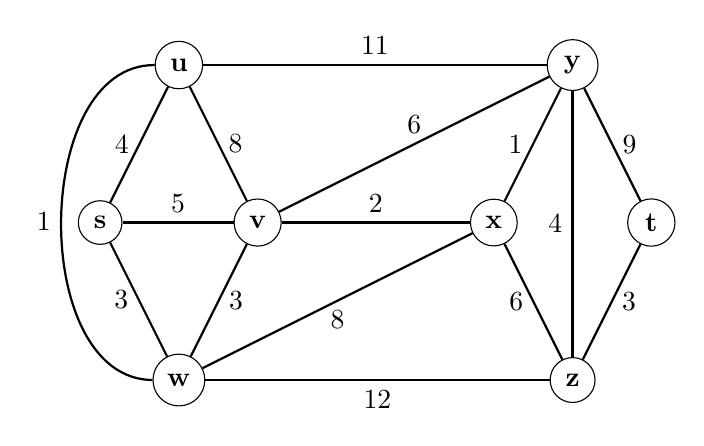
\begin{tikzpicture}

	\node[shape=circle,draw=black] (s) at (-1, 2)    {\textbf{s}};
	\node[shape=circle,draw=black] (u) at (0, 4)     {\textbf{u}};
	\node[shape=circle,draw=black] (y) at (5, 4)     {\textbf{y}};
	\node[shape=circle,draw=black] (w) at (0, 0)     {\textbf{w}};
	\node[shape=circle,draw=black] (z) at (5, 0)     {\textbf{z}};
	\node[shape=circle,draw=black] (v) at (1, 2)     {\textbf{v}};
    \node[shape=circle,draw=black] (x) at (4, 2)     {\textbf{x}};
    \node[shape=circle,draw=black] (t) at (6, 2)     {\textbf{t}};

	\path[-, thick] (u) edge [bend right=90] node[left]{1} (w);
	\path[-, thick] (s) edge node[left]{4} (u);
	\path[-, thick] (s) edge node[above]{5} (v);
	\path[-, thick] (u) edge node[right]{8} (v);
	\path[-, thick] (s) edge node[left]{3} (w);
	\path[-, thick] (v) edge node[right]{3} (w);
	\path[-, thick] (u) edge node[above]{11} (y);
	\path[-, thick] (y) edge node[right]{9} (t);
	\path[-, thick] (y) edge node[left]{1} (x);
	\path[-, thick] (y) edge node[left]{4} (z);
	\path[-, thick] (x) edge node[left]{6} (z);
	\path[-, thick] (t) edge node[right]{3} (z);
	\path[-, thick] (w) edge node[below]{12} (z);
	\path[-, thick] (x) edge node[below]{8} (w);
	\path[-, thick] (v) edge node[above]{2} (x);
	\path[-, thick] (v) edge node[above]{6} (y);

	\end{tikzpicture}
\end{figure}

\newpage

Let the distance to the starting vertex be zero.
For all vertices other than the starting vertex, if they have an edge with the starting vertex, make the distance to them equal to the weight of that edge, otherwise mark the distance as infinity.
Let the parent vertex of all vertices that have an edge with the starting vertex be the starting vertex.
The parent vertex of the starting vertex is undefined, and the parent vertex of all other vertices are yet to be determined.

\begin{figure}[H]
	\centering
    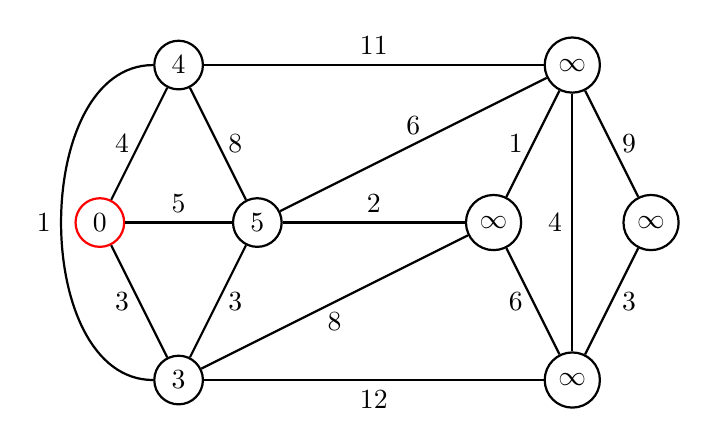
\begin{tikzpicture}[
        auto,
        semithick % line style
    ]
    \tikzstyle{every state}=[
        draw = black,
        thick,
        fill = white,
        minimum size = 4mm,
        circle
    ]

    \tikzstyle{red state}=[
        draw = red,
        thick,
        fill = white,
        minimum size = 4mm,
        circle
    ]

	\node[red state]   (s) at (-1, 2)    {0};
	\node[every state] (u) at (0, 4)     {4};
	\node[every state] (y) at (5, 4)     {$\infty$};
	\node[every state] (w) at (0, 0)     {3};
	\node[every state] (z) at (5, 0)     {$\infty$};
	\node[every state] (v) at (1, 2)     {5};
    \node[every state] (x) at (4, 2)     {$\infty$};
    \node[every state] (t) at (6, 2)     {$\infty$};

	\path[-, thick] (u) edge [bend right=90] node[left]{1} (w);
	\path[-, thick] (s) edge node[left]{4} (u);
	\path[-, thick] (s) edge node[above]{5} (v);
	\path[-, thick] (u) edge node[right]{8} (v);
	\path[-, thick] (s) edge node[left]{3} (w);
	\path[-, thick] (v) edge node[right]{3} (w);
	\path[-, thick] (u) edge node[above]{11} (y);
	\path[-, thick] (y) edge node[right]{9} (t);
	\path[-, thick] (y) edge node[left]{1} (x);
	\path[-, thick] (y) edge node[left]{4} (z);
	\path[-, thick] (x) edge node[left]{6} (z);
	\path[-, thick] (t) edge node[right]{3} (z);
	\path[-, thick] (w) edge node[below]{12} (z);
	\path[-, thick] (x) edge node[below]{8} (w);
	\path[-, thick] (v) edge node[above]{2} (x);
	\path[-, thick] (v) edge node[above]{6} (y);

	\end{tikzpicture}
\end{figure}

Since the vertex with the smallest distance is \textbf{w}, visit \textbf{w} and update the distances of \textbf{x} and \textbf{z} to be the sum of the distance of \textbf{w} and the weight of the edge between \textbf{w} and that vertex.
Mark the parent vertex of \textbf{w} as \textbf{s}.
The distance of \textbf{v} is not updated since the sum of the distance of \textbf{w} and the weight of the edge between \textbf{w} and \textbf{v}, which is 6, is greater than the current distance of \textbf{v}, which is 5.

\begin{figure}[H]
	\centering
    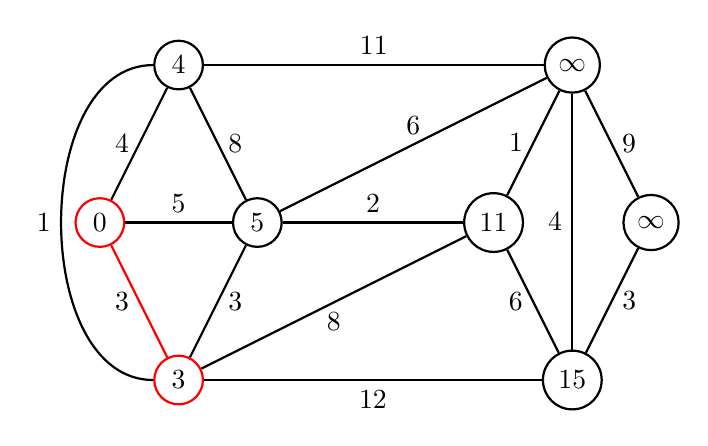
\begin{tikzpicture}
    \tikzstyle{every state}=[
        draw = black,
        thick,
        fill = white,
        minimum size = 4mm,
        circle
    ]
    \tikzstyle{red state}=[
        draw = red,
        thick,
        fill = white,
        minimum size = 4mm,
        circle
    ]

	\node[red state]   (s) at (-1, 2)    {0};
	\node[every state] (u) at (0, 4)     {4};
	\node[every state] (y) at (5, 4)     {$\infty$};
	\node[red state]   (w) at (0, 0)     {3};
	\node[every state] (z) at (5, 0)     {15};
	\node[every state] (v) at (1, 2)     {5};
    \node[every state] (x) at (4, 2)     {11};
    \node[every state] (t) at (6, 2)     {$\infty$};

	\path[-, thick] (u) edge [bend right=90] node[left]{1} (w);
	\path[-, thick] (s) edge node[left]{4} (u);
	\path[-, thick] (s) edge node[above]{5} (v);
	\path[-, thick] (u) edge node[right]{8} (v);
	\draw[-, thick] (s) edge [red] node[black, left]{3} (w);
	\path[-, thick] (v) edge node[right]{3} (w);
	\path[-, thick] (u) edge node[above]{11} (y);
	\path[-, thick] (y) edge node[right]{9} (t);
	\path[-, thick] (y) edge node[left]{1} (x);
	\path[-, thick] (y) edge node[left]{4} (z);
	\path[-, thick] (x) edge node[left]{6} (z);
	\path[-, thick] (t) edge node[right]{3} (z);
	\path[-, thick] (w) edge node[below]{12} (z);
	\path[-, thick] (x) edge node[below]{8} (w);
	\path[-, thick] (v) edge node[above]{2} (x);
	\path[-, thick] (v) edge node[above]{6} (y);

	\end{tikzpicture}
\end{figure}

\newpage

Since the unvisited vertex with the smallest distance is \textbf{u}, visit \textbf{u} and repeat the steps above.

\begin{figure}[H]
	\centering
    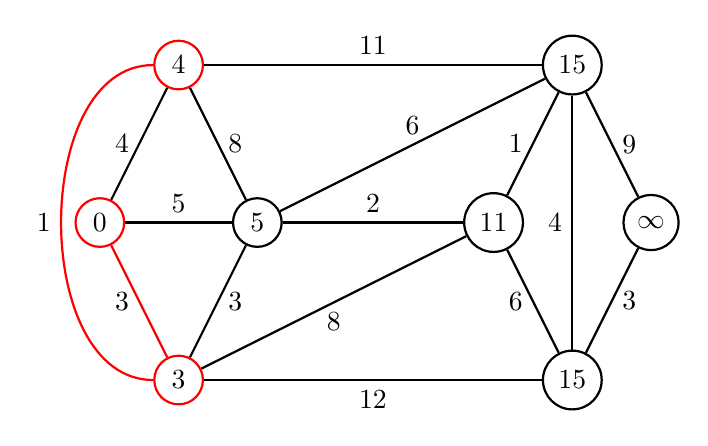
\begin{tikzpicture}
    \tikzstyle{every state}=[
        draw = black,
        thick,
        fill = white,
        minimum size = 4mm,
        circle
    ]
    \tikzstyle{red state}=[
        draw = red,
        thick,
        fill = white,
        minimum size = 4mm,
        circle
    ]

	\node[red state]   (s) at (-1, 2)    {0};
	\node[red state]   (u) at (0, 4)     {4};
	\node[every state] (y) at (5, 4)     {15};
	\node[red state]   (w) at (0, 0)     {3};
	\node[every state] (z) at (5, 0)     {15};
	\node[every state] (v) at (1, 2)     {5};
    \node[every state] (x) at (4, 2)     {11};
    \node[every state] (t) at (6, 2)     {$\infty$};

	\path[-, thick] (u) edge [red] [bend right=90] node[black, left]{1} (w);
	\path[-, thick] (s) edge node[left]{4} (u);
	\path[-, thick] (s) edge node[above]{5} (v);
	\path[-, thick] (u) edge node[right]{8} (v);
	\draw[-, thick] (s) edge [red] node[black, left]{3} (w);
	\path[-, thick] (v) edge node[right]{3} (w);
	\path[-, thick] (u) edge node[above]{11} (y);
	\path[-, thick] (y) edge node[right]{9} (t);
	\path[-, thick] (y) edge node[left]{1} (x);
	\path[-, thick] (y) edge node[left]{4} (z);
	\path[-, thick] (x) edge node[left]{6} (z);
	\path[-, thick] (t) edge node[right]{3} (z);
	\path[-, thick] (w) edge node[below]{12} (z);
	\path[-, thick] (x) edge node[below]{8} (w);
	\path[-, thick] (v) edge node[above]{2} (x);
	\path[-, thick] (v) edge node[above]{6} (y);

	\end{tikzpicture}
\end{figure}

Visit the vertex \textbf{v} and repeat the steps above.
Since its parent vertex was \textbf{s}, one must “color” the edge between \textbf{s} and \textbf{v}, not any other edge.
This step is crucial to generate the correct shortest path from the starting vertex to the ending vertex.

\begin{figure}[H]
	\centering
    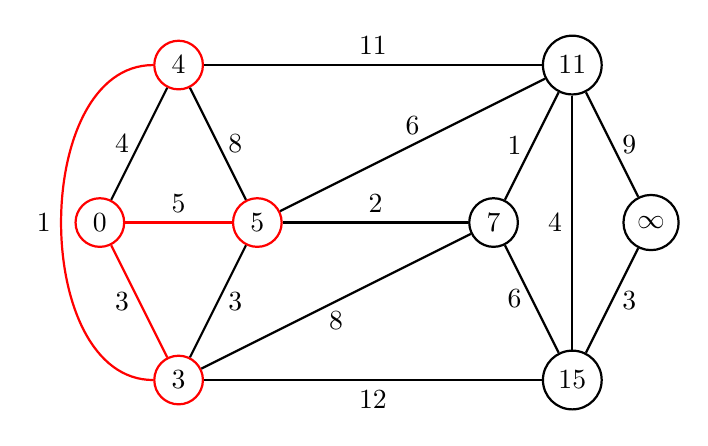
\begin{tikzpicture}
    \tikzstyle{every state}=[
        draw = black,
        thick,
        fill = white,
        minimum size = 4mm,
        circle
    ]
    \tikzstyle{red state}=[
        draw = red,
        thick,
        fill = white,
        minimum size = 4mm,
        circle
    ]

	\node[red state]   (s) at (-1, 2)    {0};
	\node[red state]   (u) at (0, 4)     {4};
	\node[every state] (y) at (5, 4)     {11};
	\node[red state]   (w) at (0, 0)     {3};
	\node[every state] (z) at (5, 0)     {15};
	\node[red state]   (v) at (1, 2)     {5};
    \node[every state] (x) at (4, 2)     {7};
    \node[every state] (t) at (6, 2)     {$\infty$};

	\path[-, thick] (u) edge [red] [bend right=90] node[black, left]{1} (w);
	\path[-, thick] (s) edge node[left]{4} (u);
	\path[-, thick] (s) edge [red] node[black, above]{5} (v);
	\path[-, thick] (u) edge node[right]{8} (v);
	\draw[-, thick] (s) edge [red] node[black, left]{3} (w);
	\path[-, thick] (v) edge node[right]{3} (w);
	\path[-, thick] (u) edge node[above]{11} (y);
	\path[-, thick] (y) edge node[right]{9} (t);
	\path[-, thick] (y) edge node[left]{1} (x);
	\path[-, thick] (y) edge node[left]{4} (z);
	\path[-, thick] (x) edge node[left]{6} (z);
	\path[-, thick] (t) edge node[right]{3} (z);
	\path[-, thick] (w) edge node[below]{12} (z);
	\path[-, thick] (x) edge node[below]{8} (w);
	\path[-, thick] (v) edge node[above]{2} (x);
	\path[-, thick] (v) edge node[above]{6} (y);

	\end{tikzpicture}
\end{figure}

Visit the vertex \textbf{x} and repeat the steps above.

\begin{figure}[H]
	\centering
    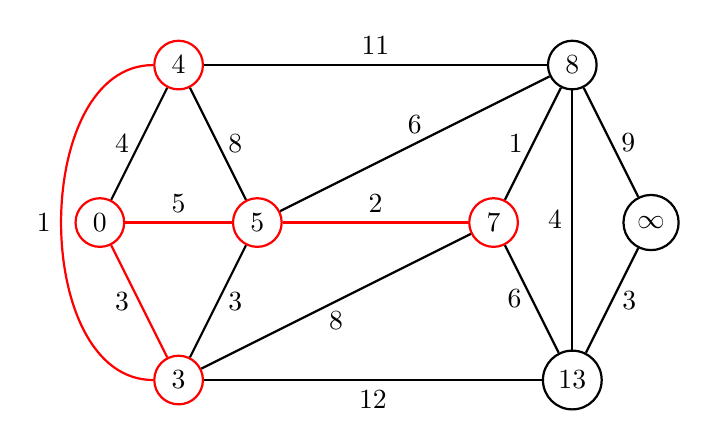
\begin{tikzpicture}
    \tikzstyle{every state}=[
        draw = black,
        thick,
        fill = white,
        minimum size = 4mm,
        circle
    ]
    \tikzstyle{red state}=[
        draw = red,
        thick,
        fill = white,
        minimum size = 4mm,
        circle
    ]

	\node[red state]   (s) at (-1, 2)    {0};
	\node[red state]   (u) at (0, 4)     {4};
	\node[every state] (y) at (5, 4)     {8};
	\node[red state]   (w) at (0, 0)     {3};
	\node[every state] (z) at (5, 0)     {13};
	\node[red state]   (v) at (1, 2)     {5};
    \node[red state]   (x) at (4, 2)     {7};
    \node[every state] (t) at (6, 2)     {$\infty$};

	\path[-, thick] (u) edge [red] [bend right=90] node[black, left]{1} (w);
	\path[-, thick] (s) edge node[left]{4} (u);
	\path[-, thick] (s) edge [red] node[black, above]{5} (v);
	\path[-, thick] (u) edge node[right]{8} (v);
	\draw[-, thick] (s) edge [red] node[black, left]{3} (w);
	\path[-, thick] (v) edge node[right]{3} (w);
	\path[-, thick] (u) edge node[above]{11} (y);
	\path[-, thick] (y) edge node[right]{9} (t);
	\path[-, thick] (y) edge node[left]{1} (x);
	\path[-, thick] (y) edge node[left]{4} (z);
	\path[-, thick] (x) edge node[left]{6} (z);
	\path[-, thick] (t) edge node[right]{3} (z);
	\path[-, thick] (w) edge node[below]{12} (z);
	\path[-, thick] (x) edge node[below]{8} (w);
	\path[-, thick] (v) edge [red] node[black, above]{2} (x);
	\path[-, thick] (v) edge node[above]{6} (y);

	\end{tikzpicture}
\end{figure}

\newpage

Visit the vertex \textbf{y} and repeat the steps above.

\begin{figure}[H]
	\centering
    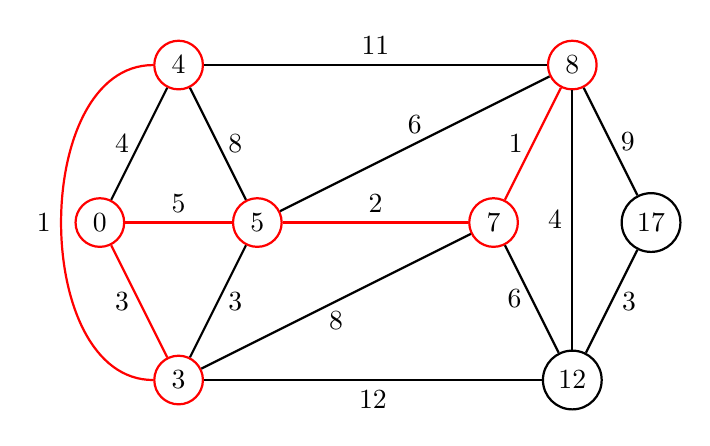
\begin{tikzpicture}
    \tikzstyle{every state}=[
        draw = black,
        thick,
        fill = white,
        minimum size = 4mm,
        circle
    ]
    \tikzstyle{red state}=[
        draw = red,
        thick,
        fill = white,
        minimum size = 4mm,
        circle
    ]

	\node[red state]   (s) at (-1, 2)    {0};
	\node[red state]   (u) at (0, 4)     {4};
	\node[red state]   (y) at (5, 4)     {8};
	\node[red state]   (w) at (0, 0)     {3};
	\node[every state] (z) at (5, 0)     {12};
	\node[red state]   (v) at (1, 2)     {5};
    \node[red state]   (x) at (4, 2)     {7};
    \node[every state] (t) at (6, 2)     {17};

	\path[-, thick] (u) edge [red] [bend right=90] node[black, left]{1} (w);
	\path[-, thick] (s) edge node[left]{4} (u);
	\path[-, thick] (s) edge [red] node[black, above]{5} (v);
	\path[-, thick] (u) edge node[right]{8} (v);
	\draw[-, thick] (s) edge [red] node[black, left]{3} (w);
	\path[-, thick] (v) edge node[right]{3} (w);
	\path[-, thick] (u) edge node[above]{11} (y);
	\path[-, thick] (y) edge node[right]{9} (t);
	\path[-, thick] (y) edge [red] node[black, left]{1} (x);
	\path[-, thick] (y) edge node[left]{4} (z);
	\path[-, thick] (x) edge node[left]{6} (z);
	\path[-, thick] (t) edge node[right]{3} (z);
	\path[-, thick] (w) edge node[below]{12} (z);
	\path[-, thick] (x) edge node[below]{8} (w);
	\path[-, thick] (v) edge [red] node[black, above]{2} (x);
	\path[-, thick] (v) edge node[above]{6} (y);

	\end{tikzpicture}
\end{figure}

Visit the vertex \textbf{z} and repeat the steps above.

\begin{figure}[H]
	\centering
    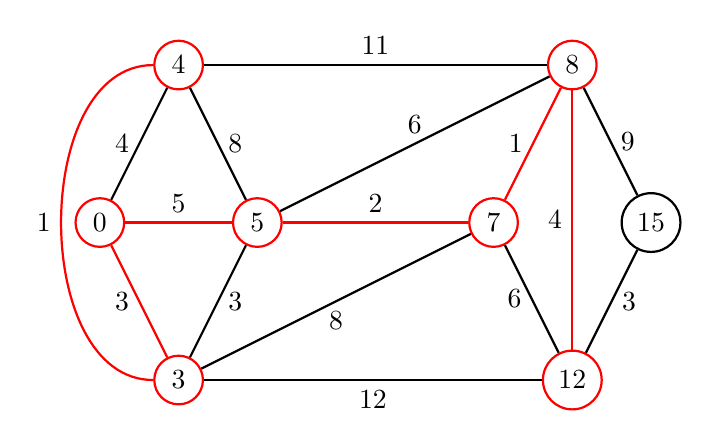
\begin{tikzpicture}
    \tikzstyle{every state}=[
        draw = black,
        thick,
        fill = white,
        minimum size = 4mm,
        circle
    ]
    \tikzstyle{red state}=[
        draw = red,
        thick,
        fill = white,
        minimum size = 4mm,
        circle
    ]

	\node[red state]   (s) at (-1, 2)    {0};
	\node[red state]   (u) at (0, 4)     {4};
	\node[red state]   (y) at (5, 4)     {8};
	\node[red state]   (w) at (0, 0)     {3};
	\node[red state]   (z) at (5, 0)     {12};
	\node[red state]   (v) at (1, 2)     {5};
    \node[red state]   (x) at (4, 2)     {7};
    \node[every state] (t) at (6, 2)     {15};

	\path[-, thick] (u) edge [red] [bend right=90] node[black, left]{1} (w);
	\path[-, thick] (s) edge node[left]{4} (u);
	\path[-, thick] (s) edge [red] node[black, above]{5} (v);
	\path[-, thick] (u) edge node[right]{8} (v);
	\draw[-, thick] (s) edge [red] node[black, left]{3} (w);
	\path[-, thick] (v) edge node[right]{3} (w);
	\path[-, thick] (u) edge node[above]{11} (y);
	\path[-, thick] (y) edge node[right]{9} (t);
	\path[-, thick] (y) edge [red] node[black, left]{1} (x);
	\path[-, thick] (y) edge [red] node[black, left]{4} (z);
	\path[-, thick] (x) edge node[left]{6} (z);
	\path[-, thick] (t) edge node[right]{3} (z);
	\path[-, thick] (w) edge node[below]{12} (z);
	\path[-, thick] (x) edge node[below]{8} (w);
	\path[-, thick] (v) edge [red] node[black, above]{2} (x);
	\path[-, thick] (v) edge node[above]{6} (y);

	\end{tikzpicture}
\end{figure}

Visit the vertex \textbf{t} and halt the algorithm, since we visited the desired ending vertex.

\begin{figure}[H]
	\centering
    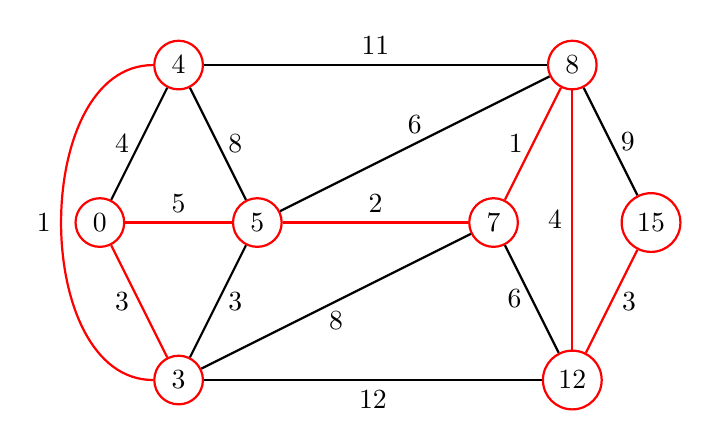
\begin{tikzpicture}
    \tikzstyle{every state}=[
        draw = black,
        thick,
        fill = white,
        minimum size = 4mm,
        circle
    ]
    \tikzstyle{red state}=[
        draw = red,
        thick,
        fill = white,
        minimum size = 4mm,
        circle
    ]

	\node[red state]   (s) at (-1, 2)    {0};
	\node[red state]   (u) at (0, 4)     {4};
	\node[red state]   (y) at (5, 4)     {8};
	\node[red state]   (w) at (0, 0)     {3};
	\node[red state]   (z) at (5, 0)     {12};
	\node[red state]   (v) at (1, 2)     {5};
    \node[red state]   (x) at (4, 2)     {7};
    \node[red state]   (t) at (6, 2)     {15};

	\path[-, thick] (u) edge [red] [bend right=90] node[black, left]{1} (w);
	\path[-, thick] (s) edge       node[left]{4} (u);
	\path[-, thick] (s) edge [red] node[black, above]{5} (v);
	\path[-, thick] (u) edge       node[right]{8} (v);
	\draw[-, thick] (s) edge [red] node[black, left]{3} (w);
	\path[-, thick] (v) edge       node[right]{3} (w);
	\path[-, thick] (u) edge       node[above]{11} (y);
	\path[-, thick] (y) edge       node[right]{9} (t);
	\path[-, thick] (y) edge [red] node[black, left]{1} (x);
	\path[-, thick] (y) edge [red] node[black, left]{4} (z);
	\path[-, thick] (x) edge       node[left]{6} (z);
	\path[-, thick] (t) edge [red] node[black, right]{3} (z);
	\path[-, thick] (w) edge       node[below]{12} (z);
	\path[-, thick] (x) edge       node[below]{8} (w);
	\path[-, thick] (v) edge [red] node[black, above]{2} (x);
	\path[-, thick] (v) edge       node[above]{6} (y);

	\end{tikzpicture}
\end{figure}

Therefore, the shortest path between the vertex \textbf{s} and the vertex \textbf{t} is $(\textbf{s}, \textbf{v}, \textbf{x}, \textbf{y}, \textbf{z}, \textbf{t})$ and its length is 15.

\newpage

\section*{Answer 4}


\end{document}